\section{Gaussian importance sampling for state space models}
\label{sec:gaussian_importance_sampling_for_state_space_models}

% two types of proposals: direct, SSMs
For the types of models considered in this thesis, importance sampling is used to infer the posterior distribution. Given a state space model of the form \eqref{def:ssm} and observations $Y = Y_{:n}$, let $\P$ be the distribution of the states $X=X_{:n}$, conditional on $Y$ and $f$ be a function of interest. The task at hand is now to find a suitable proposal $\G$, using the methods presented in the last section. If $n$ is large, the posterior distribution lives in a high dimensional state of dimension $m\cdot n$ so to obtain $\G$ efficiently, we should exploit the available structure. Additionally, we want $\G$ to be tractable, so simulating from it is possible and evaluating the weights $w$ up to a constant is possible. 

The multivariate Gaussian distribution is a good candidate in this setting, as simulating from it is straightforward and its density can be evaluated analytically. However, naively performing the optimal importance sampling methods from the previous section for all multivariate Gaussians is computationally inefficient as the family of distributions has $\mathcal O((n\cdot m)^{2})$ many parameters. We can, however, exploit the available structure of the \gls{ssm} to find parametrizations with fewer parameters. 

% first: Gaussian SSMs
The first approach \todo{cite} is motivated by the fact that the target posterior is again a Markov process, as are posteriors in \glspl{glssm}. Additionally, the posterior distribution in \gls{glssm}s is again Gaussian, and straightforward to simulate from by, e.g., the FFBS \todo{cite} algorithm. Thus parameterizing the proposals $\G$ by the posterior of a suitably chosen \gls{glssm} may be a fruitful approach.
For the models we consider in this thesis, the distribution of states is already Gaussian and the observations are conditionally independent given the states. Thus a natural \gls{glssm} to use as a proposal consists of keeping the prior distribution of states and replacing the distribution of observations with conditionally independent Gaussian distributions and the actual observations by synthetic ones. By the assumed conditional independence, this model only needs $2 p\cdot (n + 1)$ many parameters, $p\cdot (n + 1)$ for the synthetic observations and $p\cdot (n + 1)$ for their variances. We term this approach the \textbf{\gls{glssm}-approach} to importance sampling.

In total, the \gls{glssm}-approach considers parametric proposals $\G_{\psi}$ of the form
\begin{align}
    \begin{split}
    \label{eq:glssm-proposal}
    \G_{\psi} &= \mathcal L(X | Z = z),\\
    Z_{t} &= B_{t} X_{t} + \eta_{t},\\
    \eta_{t} &\sim \mathcal N \left( 0, \Omega_{t} \right),\\
    \Omega_{t} &= \diag \left( \omega^{2}_{t} \right) = \diag \left( \omega^{2}_{t,1}, \dots, \omega^{2}_{1,p} \right).
    \end{split}
\end{align}
where the distribution of $X$ is given by \eqref{eq:glssm_states}, $\psi = \left( z, \omega^{2} \right)$ for $z = \left( z_{0}, \dots, z_{n} \right) \in \R^{n \times m}$ and $\omega^{2} = \left( \omega^{2}_{0}, \dots, \omega^{2}_{n} \right) \in \R^{n \times m}$. Alternatively the natural parametrization $\psi = \left( z \oslash \omega^{2}, - 1 \oslash \left( 2 \omega^{2} \right) \right)$ may also be used, where $\oslash$ is the Hadamard, i.e. entry-wise, division. Simulation from $\G_{\psi}$ may be efficiently implemented by the FFBS algorithm, as $\G_{\psi}$ is the smoothing distribution of a \gls{glssm}. 

% weights
In this setting, the importance sampling weights are given by 
$$
w(x) = \frac{p(x|y)}{g(x|z)} = \frac{p(y|x)p(x)}{g(z|x)p(x)} \frac{g(z)}{p(y)} \propto \prod_{t = 0}^n \frac{p(y_{t}|x_{t})}{g(z_{t}|x_{t})},
$$
% Signals
so they can be computed efficiently. Additionally, as \todo{add signal restriction above} $p(y_{t}|x_{t})$ and $g(z_{t}|x_{t})$ depend on $x_{t}$ only through the signal $s_{t} = B_{t}x_{t}$, we have 
$$
w(x) \propto \prod_{t = 0}^{n}\frac{p(y_{t}|s_{t})}{g(z_{t}|s_{t})},
$$
which implies that auto-normalized weights may be calculated by using the signal smoother \cite[Theorem 2]{Jungbacker2007Monte}.
\todo{introduce LCSSM with linear signals above}
As \citeauthor{Durbin2012Time} \cite[Section 4.5.3]{Durbin2012Time} argue, it is often computationally more efficient to treat only on the signals $\left(S_{t}\right)_{t=0,\dots,n}$ instead of the states $ \left( X_{t}  \right)_{t = 0, \dots, n}$, the idea being that the dimension of $S_{t}$, $p$, is usually much smaller than that of $X_{t}$, $m$. 

% sample from states still possbile if doingo nly signals, weights don't change
As the joint distribution of $(X, S)$ is a Gaussian distribution, by \Cref{lem:gaussian_conditional} $X|S = s$ is again Gaussian \todo{add degernate case to gaussian conditional lemma}, with known conditional mean and covariance matrix and density $p(x|s) = g(x|s)$. If $(\tilde X_{t})_{t=0,\dots,n}$ is a draw from this conditional distribution a quick calculation reveals that a.s. $B_{t} \tilde X_{t} = S_{t}$, and so, as expected, the weights $w(\tilde X)$ are a.s. constant and given by (up to the integration constant) $\prod_{t = 0}^{n}\frac{p(y_{t}|s_{t})}{g(y_{t}|s_{t})}$. Producing a draw from this conditional distribution can be achieved by the FFBS algorithm \Cref{alg:ffbs}, as $(X, S)$ form a \gls{glssm} with degenerate observation covariance matrices $\Omega_{t} = 0$.

By the assumed conditional independence of observations given signals, we have
$$
p(x, s|y) \propto p(x|s) p(s|y),
$$
and so if one is interested in the states, rather than the signals, importance sampling with the proposal \Cref{eq:glssm-proposal} can be achieved in a two-step procedure: first sample from $g(s|z)$, then run the FFBS algorithm to sample from $g(x|s) = p(x|s)$ using the same weights for MC-integration. 

% degenerate distribution, exponential family of proposals for signals


\todo{initroduce signals, importance sampling only w.r.t. signals. What if signal covariance matrix is degenerated?}
\todo{probably cite something about curved exponential families, e.g. Brown1986Fundamentals}

The \gls{glssm}-approach is the standard approach for finding the \gls{la} in \gls{lcssm} \cite{Durbin1997Monte,Durbin2012Time,Jungbacker2007Monte} and also leads to efficient implementation for \gls{eis} \cite{Koopman2019Modified}. However, as will become apparent in the later part of this section, this approach is infeasible for the \gls{cem} if $n$ is large. 

% second: Gaussian Markov process 
% discuss more flexible vs. fewer parameters
An alternative family of Gaussian proposals, is given by directly modeling a Gaussian Markov process on the states $X_{:n}$. Again, this is sensible given the Markov structure of the target. This parametrization is more flexible than using the posterior of a \gls{glssm} with fixed prior as the proposal. This flexibility, however, comes at the cost of requiring a larger number of parameters. Here we propose with $\G_{\psi}$ where
\begin{align}
    \begin{split}
    \label{eq:markov-proposal}
    \G_{\psi} &= \mathcal L (U) \\
    U_{0} &\sim \mathcal N(v_{0}, \Xi_{0})\\
    U_{t} &= C_{t}U_{t - 1} + v_{t} + \nu_{t} \\
    v_{t} \in \R^{m}, &C_{t} \in \R^{m\times m}\\
    \nu_{t} &\sim \mathcal N(0,\Xi_{t}) \\
    &\Xi_{t}\in\R^{m \times m} \text{ positive definite}
    \end{split}
\end{align}
for $t = 1, \dots, n$, with $U_{0}$ and $\nu_{1}, \dots, \nu_{n}$ independent. The number of parameters is $(n + 1)\cdot m$ for the means $v_{0}, \dots, v_{n + 1}$, $n \cdot m^{2}$ for the transition matrices $C_{t}$ and $(n + 1) \frac{m (m - 1)}{2}$ for the covariance matrices of innvoations, totalling $\mathcal O(n\cdot m^{2})$ many parameters. 
While these are considerably more parameters for large state dimension $m$, we will see that finding the optimal parameters for the \gls{cem} can be done analytically \todo{cite relevant section}. Simulation from $\G_{\psi}$ is achieved by a simple recursion. 
This approach, which we term the \textbf{Markov-approach}, was originally proposed by \citeauthor{Richard2007Efficient} in \cite{Richard2007Efficient} for general unnormalized transition kernels as \gls{eis} proposals.

% discuss if there actually is a Gaussian close to the target, see heavy tails etc.
Using Gaussian proposals, while computationally efficient, also comes with some drawbacks. The whole procedure hinges on the assumption that there is a Gaussian that is, close to the target distribution. In the setting of \glspl{ssm} this is not guaranteed, as the targets may contain multiple modes or heavy tails, features that may, in the worst case, lead to inconsistent importance sampling estimates. At least for the models considered in \Cref{cha:analysis_of_selected_models}, the targets arise as posterior distributions of \gls{lcssm} and as such they are unimodal and have non-heavy tails, i.e. there is a Gaussian distribution such that importance sampling is feasible \todo{rethink, is this really the case, for LCSSM it depends on log-partition function of observations}. 
Additionally, even if there is a Gaussian distribution that facilitates consistent importance sampling, finding it in practice may be complicated, as the proposals generated by the \gls{la}, \gls{cem} and \gls{eis} have deteriorating performance for fixed sample size $N$ (in terms of \gls{ess} and convergence) with increasing dimension \todo{ref to chapter, check that I also present that there}.

We now give a concise overview over how to perform the \gls{la} and \gls{eis} for \gls{lcssm}, but refer the reader for more details to the respective literature.
The \gls{la} \todo{...}
% SSMs may utilize KF/KS to perform importance sampling
% LA: cite Koopman paper
% EIS: cite papers, MEIS NEIS


% CE: two variants 
%% GLSSM approach fails: 
For the \gls{cem}, using the \gls{glssm}-approach turns out to be difficult numerically. For a high-level argument of why this is true, let us ignore the Markov structure of the model for the moment. As the \gls{cem} matches moments of the target and proposal, applying it to fit model \eqref{eq:glssm-proposal} amounts to matching the moments of $\G_{\psi}$ to those of the target posterior $\mathcal L (X | Y = y)$ in the \gls{ssm}. Unfortunately, the covariance of $\G_{\psi}$ is given by $ \left( \Sigma^{-1} + B^{T}\Omega^{-1} B \right)^{-1}$, where $\Sigma$ is the covariance of all states, $B = \bdiag (B_{0}, \dots, B_{n})$ and $\Omega = \bdiag \left( \Omega_{0}, \dots, \Omega_{n} \right)$. Choosing the diagonal matrix $\Omega$ such that the covariance of $\G_{\psi}$ matches this expression is numerically expensive: we either need to invert the large (dimension $(n + 1)m \times (n + 1)m$) covariance matrix, or solve numerically for the $(n + 1)p$ parameters. The problem at hand is that we cannot decouple this into $(n + 1)$ equations of dimension $p$, as all entries of $(\Sigma^{-1} + B^{T}\Omega^{-1} B)^{-1}$ depend on all entries of $\Omega$. 

To make matters more concrete, the \gls{cem} finds $\psi = (z, \omega^{2})$ such that model \eqref{eq:glssm-proposal} maximizes the cross entropy with the target $\P^{X|Y=y}$. For simplicity, let us assume that $m = p$, $B$ is the identity and we only observe a single $y$. Using \Cref{lem:gaussian_conditional}, we see that when $X\sim\mathcal N(\mu, \Sigma)$, the conditional distribution of $X$ given $Z=z$, $\G_{\psi}$, is a Gaussian distribution with mean $\tilde \mu =  \mu + \Sigma \left( \Sigma  + \Omega \right)^{-1} \left( z - \mu \right)$  and covariance matrix $\tilde\Sigma = \left( \Sigma ^{-1} + \Omega^{-1}\right)^{-1}$ for $\Omega = \diag \left( \omega^{2} \right)$, where $\omega^{2} > 0$. Assuming that $\Sigma$ is non-singular, we can reparameterize the objective function of the \gls{cem} by $\tilde \mu$,
\begin{align*}
\max_{z, \omega^{2}} \int p(x|y) \log g_{\psi}(x|z) \mathrm dx &= \max_{\tilde\mu, \omega^{2}} \int p(x|y) \left( - \frac{1}{2} (x - \tilde \mu)^{T} \tilde \Sigma ^{-1} \left( x - \tilde \mu \right)  - \frac{1}{2} \log\det \tilde \Sigma \right)  \d x\\
&= \max_{\tilde \mu, \omega^{2}} - \frac{1}{2} (\gamma - \tilde \mu)^{T}\tilde \Sigma ^{-1} ( \gamma - \tilde \mu) - \frac{1}{2} \operatorname{trace} \left( \tilde \Sigma^{-1} \Gamma \right) - \frac{1}{2} \log\det\tilde\Sigma,
\end{align*}
where $\gamma = \E \left( X | Y = y \right)$ and $\Gamma = \cov \left( X | Y = y \right)$. 
Thus the optimal $\tilde \mu$ is $\gamma$ and to find $\omega^{2}$ we have to minimize 
$$
\operatorname{trace} \left( \left( \Sigma^{-1} + \Omega^{-1} \right) \Gamma \right) - \log\det \left( \Sigma^{-1} + \Omega^{-1} \right).
$$
Taking the derivative w.r.t. $\frac{1}{\omega^{2}}$, we see that 
\begin{align}
\label{eq:gamma_post}
\Gamma_{i,i} = \left(\left( \Sigma^{-1} + \diag \left( \frac{1}{\omega_{1}}, \dots, \frac{1}{\omega_{p}}\right) \right)^{-1}\right)_{i,i} = \left( \Sigma - \Sigma \left( \Sigma + \Omega \right)^{-1}\Sigma \right)_{i,i} %= \Sigma_{i,i} - \Sigma_{i}^T \left( \Sigma + \Omega \right)^{-1} \Sigma_{i},
\end{align}
has to hold for all $i = 1, \dots, p$, i.e. we have to choose $\omega^{2}$ such that the posterior marginal variances $\Gamma_{i,i}$ coincide with the marginal variances of $\G_{\psi}$.

Several problems arise: First of all, \Cref{eq:gamma_post} is not guaranteed to have a solution. For the $i$-th unit-vector $e_{i}\in\R^{p}$ we can reformulate \Cref{eq:gamma_post} to 
$$
\Sigma_{i,i} - \Gamma_{i,i} = e_{i}^T\Sigma^{T} \left( \Sigma + \Omega \right)^{-1}\Sigma e_{i} > 0
$$
and so we require $\Gamma_{i,i} < \Sigma_{i,i}$. While the law of total covariance asserts that
$$
\Sigma = \E \underbrace{\cov \left( X | Y \right)}_{=\Gamma} + \cov \left( \E \left( X | Y \right) \right),
$$
it does not guarantee $\Gamma \prec \Sigma$, which would imply $\Gamma_{i,i} < \Sigma_{i,i}$. 
\todo{can we find example?}

Second, even if there is an analytical solution $\Omega$ to \Cref{eq:gamma_post}, in the \gls{cem} we replace $\Gamma_{i,i}$ by the observed marginal variances $\hat\Gamma_{i,i}$ obtained by importance sampling. The variation introduced by simulation can then lead to situations where $\hat\Gamma_{i,i} > \Sigma_{i,i}$. As an example take $X \sim \mathcal N(0, 1)$, and $Y = X + \eta$ for $\eta \sim \mathcal N(0, \omega^{2})$. Then the conditional variance of $X$ given $Y = y$ is $\Gamma = 1 - \frac{1}{1 + \omega^{2}}$. Given $N$ i.i.d. samples $X^{1}, \dots X^{N}$ from this distribution, their empirical variance $\hat \Gamma = \frac{1}{N} \sum_{i = 1}^{N} (X^{i} - \bar X)^{2} $ follows a scaled $\chi_{N - 1}^{2}$ distribution, i.e. $ \frac{N\hat\Gamma}{\Gamma} \sim \chi^{2}_{N - 1}$. Notice that we use the non-Bessel corrected version of the empirical variance here, as this is the maximum-likelihood estimate. 

Then $$\P \left( \hat \Gamma > 1 \right) = \P \left( \frac{N \hat \Gamma}{\Gamma} > \frac{N}{\Gamma} \right) = 1 - F_{\chi^{2}_{N-1}} \left( N \left( 1 + \frac{1}{\omega^{2}} \right) \right)$$ is the probability that \Cref{eq:gamma_post} has no solution $\omega^{2} \in \R_{\geq 0}$ \todo{introduce symbol}. Here $F_{\chi^{2}_{N - 1}}$ is the cumulative distribution function of the $\chi^{2}_{N - 1}$ distribution. As $\omega^{2}$ goes to $\infty$, this probability approaches $1 - F_{\chi^{2}_{N - 1}}(N)$ which, for large $N$, is approximately $1 - F_{\chi^{2}_{N - 1}} (N - 1) = \frac{1}{2}$. 
We illustrate this in \Cref{fig:ce_prob_failure}, displaying the probability of failure in this setting for various combinations of $N$ and $\omega^{2}$. In this figure, we see that with growing $N$ the threshold for $\omega^{2}$ leading to non-negligible failure probability becomes larger, as expected. 
Thus, even in the very simple univariate Gaussian setting, for every $N$ there is an $\omega^{2}$ such that the \gls{cem} fails for \Cref{eq:glssm-proposal} with practically relevant probability. 

\begin{figure}
    \resizebox{\textwidth}{!}{%
        % Created by tikzDevice version 0.12.6 on 2024-07-02 14:22:08
% !TEX encoding = UTF-8 Unicode
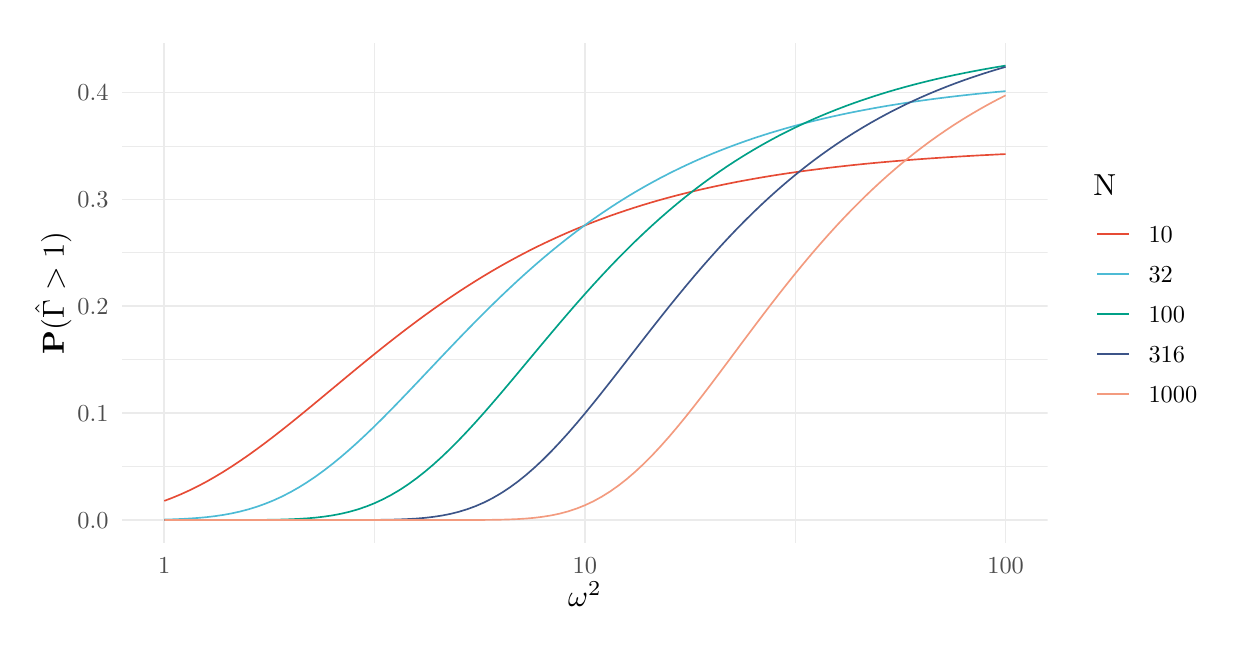
\begin{tikzpicture}[x=1pt,y=1pt]
\definecolor{fillColor}{RGB}{255,255,255}
\path[use as bounding box,fill=fillColor,fill opacity=0.00] (0,0) rectangle (433.62,216.81);
\begin{scope}
\path[clip] ( 34.16, 30.69) rectangle (368.57,211.31);
\definecolor{drawColor}{gray}{0.92}

\path[draw=drawColor,line width= 0.3pt,line join=round] ( 34.16, 58.20) --
	(368.57, 58.20);

\path[draw=drawColor,line width= 0.3pt,line join=round] ( 34.16, 96.82) --
	(368.57, 96.82);

\path[draw=drawColor,line width= 0.3pt,line join=round] ( 34.16,135.43) --
	(368.57,135.43);

\path[draw=drawColor,line width= 0.3pt,line join=round] ( 34.16,174.05) --
	(368.57,174.05);

\path[draw=drawColor,line width= 0.3pt,line join=round] (125.36, 30.69) --
	(125.36,211.31);

\path[draw=drawColor,line width= 0.3pt,line join=round] (277.37, 30.69) --
	(277.37,211.31);

\path[draw=drawColor,line width= 0.6pt,line join=round] ( 34.16, 38.90) --
	(368.57, 38.90);

\path[draw=drawColor,line width= 0.6pt,line join=round] ( 34.16, 77.51) --
	(368.57, 77.51);

\path[draw=drawColor,line width= 0.6pt,line join=round] ( 34.16,116.13) --
	(368.57,116.13);

\path[draw=drawColor,line width= 0.6pt,line join=round] ( 34.16,154.74) --
	(368.57,154.74);

\path[draw=drawColor,line width= 0.6pt,line join=round] ( 34.16,193.35) --
	(368.57,193.35);

\path[draw=drawColor,line width= 0.6pt,line join=round] ( 49.36, 30.69) --
	( 49.36,211.31);

\path[draw=drawColor,line width= 0.6pt,line join=round] (201.36, 30.69) --
	(201.36,211.31);

\path[draw=drawColor,line width= 0.6pt,line join=round] (353.37, 30.69) --
	(353.37,211.31);
\definecolor{drawColor}{RGB}{230,75,53}

\path[draw=drawColor,line width= 0.6pt,line join=round] ( 49.36, 45.81) --
	( 52.40, 46.97) --
	( 55.44, 48.24) --
	( 58.48, 49.62) --
	( 61.52, 51.12) --
	( 64.56, 52.73) --
	( 67.60, 54.46) --
	( 70.64, 56.28) --
	( 73.68, 58.21) --
	( 76.72, 60.23) --
	( 79.76, 62.33) --
	( 82.80, 64.52) --
	( 85.84, 66.77) --
	( 88.88, 69.09) --
	( 91.92, 71.46) --
	( 94.96, 73.88) --
	( 98.00, 76.34) --
	(101.04, 78.83) --
	(104.08, 81.34) --
	(107.12, 83.86) --
	(110.16, 86.39) --
	(113.20, 88.92) --
	(116.24, 91.44) --
	(119.28, 93.95) --
	(122.32, 96.44) --
	(125.36, 98.90) --
	(128.40,101.34) --
	(131.44,103.74) --
	(134.48,106.10) --
	(137.52,108.43) --
	(140.56,110.71) --
	(143.60,112.94) --
	(146.64,115.12) --
	(149.68,117.26) --
	(152.72,119.34) --
	(155.76,121.37) --
	(158.80,123.34) --
	(161.84,125.26) --
	(164.88,127.13) --
	(167.92,128.94) --
	(170.96,130.70) --
	(174.00,132.40) --
	(177.04,134.04) --
	(180.08,135.64) --
	(183.12,137.18) --
	(186.16,138.67) --
	(189.20,140.10) --
	(192.24,141.49) --
	(195.28,142.83) --
	(198.32,144.12) --
	(201.36,145.36) --
	(204.40,146.56) --
	(207.44,147.71) --
	(210.48,148.82) --
	(213.52,149.88) --
	(216.56,150.91) --
	(219.60,151.89) --
	(222.64,152.84) --
	(225.68,153.75) --
	(228.72,154.62) --
	(231.76,155.46) --
	(234.80,156.26) --
	(237.84,157.03) --
	(240.88,157.77) --
	(243.92,158.48) --
	(246.97,159.16) --
	(250.01,159.81) --
	(253.05,160.44) --
	(256.09,161.04) --
	(259.13,161.61) --
	(262.17,162.16) --
	(265.21,162.69) --
	(268.25,163.20) --
	(271.29,163.68) --
	(274.33,164.14) --
	(277.37,164.58) --
	(280.41,165.01) --
	(283.45,165.41) --
	(286.49,165.80) --
	(289.53,166.18) --
	(292.57,166.53) --
	(295.61,166.87) --
	(298.65,167.20) --
	(301.69,167.51) --
	(304.73,167.81) --
	(307.77,168.09) --
	(310.81,168.36) --
	(313.85,168.62) --
	(316.89,168.87) --
	(319.93,169.11) --
	(322.97,169.34) --
	(326.01,169.56) --
	(329.05,169.76) --
	(332.09,169.96) --
	(335.13,170.15) --
	(338.17,170.34) --
	(341.21,170.51) --
	(344.25,170.68) --
	(347.29,170.83) --
	(350.33,170.99) --
	(353.37,171.13);
\definecolor{drawColor}{RGB}{77,187,213}

\path[draw=drawColor,line width= 0.6pt,line join=round] ( 49.36, 39.07) --
	( 52.40, 39.15) --
	( 55.44, 39.27) --
	( 58.48, 39.44) --
	( 61.52, 39.65) --
	( 64.56, 39.93) --
	( 67.60, 40.29) --
	( 70.64, 40.74) --
	( 73.68, 41.29) --
	( 76.72, 41.96) --
	( 79.76, 42.76) --
	( 82.80, 43.69) --
	( 85.84, 44.78) --
	( 88.88, 46.01) --
	( 91.92, 47.41) --
	( 94.96, 48.97) --
	( 98.00, 50.70) --
	(101.04, 52.59) --
	(104.08, 54.64) --
	(107.12, 56.85) --
	(110.16, 59.20) --
	(113.20, 61.69) --
	(116.24, 64.31) --
	(119.28, 67.04) --
	(122.32, 69.88) --
	(125.36, 72.81) --
	(128.40, 75.82) --
	(131.44, 78.90) --
	(134.48, 82.03) --
	(137.52, 85.20) --
	(140.56, 88.39) --
	(143.60, 91.61) --
	(146.64, 94.82) --
	(149.68, 98.04) --
	(152.72,101.23) --
	(155.76,104.41) --
	(158.80,107.55) --
	(161.84,110.65) --
	(164.88,113.71) --
	(167.92,116.71) --
	(170.96,119.66) --
	(174.00,122.55) --
	(177.04,125.38) --
	(180.08,128.14) --
	(183.12,130.83) --
	(186.16,133.45) --
	(189.20,136.00) --
	(192.24,138.47) --
	(195.28,140.87) --
	(198.32,143.20) --
	(201.36,145.45) --
	(204.40,147.63) --
	(207.44,149.74) --
	(210.48,151.77) --
	(213.52,153.74) --
	(216.56,155.63) --
	(219.60,157.46) --
	(222.64,159.22) --
	(225.68,160.91) --
	(228.72,162.55) --
	(231.76,164.11) --
	(234.80,165.62) --
	(237.84,167.07) --
	(240.88,168.47) --
	(243.92,169.81) --
	(246.97,171.09) --
	(250.01,172.32) --
	(253.05,173.51) --
	(256.09,174.64) --
	(259.13,175.73) --
	(262.17,176.78) --
	(265.21,177.78) --
	(268.25,178.74) --
	(271.29,179.65) --
	(274.33,180.54) --
	(277.37,181.38) --
	(280.41,182.19) --
	(283.45,182.96) --
	(286.49,183.70) --
	(289.53,184.41) --
	(292.57,185.09) --
	(295.61,185.74) --
	(298.65,186.36) --
	(301.69,186.95) --
	(304.73,187.52) --
	(307.77,188.07) --
	(310.81,188.59) --
	(313.85,189.08) --
	(316.89,189.56) --
	(319.93,190.02) --
	(322.97,190.45) --
	(326.01,190.87) --
	(329.05,191.27) --
	(332.09,191.65) --
	(335.13,192.01) --
	(338.17,192.36) --
	(341.21,192.69) --
	(344.25,193.01) --
	(347.29,193.31) --
	(350.33,193.60) --
	(353.37,193.88);
\definecolor{drawColor}{RGB}{0,160,135}

\path[draw=drawColor,line width= 0.6pt,line join=round] ( 49.36, 38.90) --
	( 52.40, 38.90) --
	( 55.44, 38.90) --
	( 58.48, 38.90) --
	( 61.52, 38.90) --
	( 64.56, 38.90) --
	( 67.60, 38.90) --
	( 70.64, 38.90) --
	( 73.68, 38.90) --
	( 76.72, 38.91) --
	( 79.76, 38.92) --
	( 82.80, 38.93) --
	( 85.84, 38.96) --
	( 88.88, 39.00) --
	( 91.92, 39.07) --
	( 94.96, 39.17) --
	( 98.00, 39.31) --
	(101.04, 39.51) --
	(104.08, 39.77) --
	(107.12, 40.13) --
	(110.16, 40.58) --
	(113.20, 41.16) --
	(116.24, 41.87) --
	(119.28, 42.74) --
	(122.32, 43.77) --
	(125.36, 44.99) --
	(128.40, 46.40) --
	(131.44, 48.00) --
	(134.48, 49.80) --
	(137.52, 51.81) --
	(140.56, 54.01) --
	(143.60, 56.41) --
	(146.64, 58.99) --
	(149.68, 61.75) --
	(152.72, 64.66) --
	(155.76, 67.73) --
	(158.80, 70.92) --
	(161.84, 74.23) --
	(164.88, 77.63) --
	(167.92, 81.12) --
	(170.96, 84.67) --
	(174.00, 88.27) --
	(177.04, 91.90) --
	(180.08, 95.55) --
	(183.12, 99.20) --
	(186.16,102.84) --
	(189.20,106.46) --
	(192.24,110.05) --
	(195.28,113.60) --
	(198.32,117.10) --
	(201.36,120.53) --
	(204.40,123.91) --
	(207.44,127.21) --
	(210.48,130.45) --
	(213.52,133.60) --
	(216.56,136.67) --
	(219.60,139.66) --
	(222.64,142.56) --
	(225.68,145.38) --
	(228.72,148.11) --
	(231.76,150.75) --
	(234.80,153.31) --
	(237.84,155.78) --
	(240.88,158.17) --
	(243.92,160.47) --
	(246.97,162.69) --
	(250.01,164.83) --
	(253.05,166.89) --
	(256.09,168.87) --
	(259.13,170.77) --
	(262.17,172.60) --
	(265.21,174.36) --
	(268.25,176.05) --
	(271.29,177.68) --
	(274.33,179.24) --
	(277.37,180.73) --
	(280.41,182.16) --
	(283.45,183.54) --
	(286.49,184.86) --
	(289.53,186.12) --
	(292.57,187.33) --
	(295.61,188.49) --
	(298.65,189.60) --
	(301.69,190.66) --
	(304.73,191.68) --
	(307.77,192.65) --
	(310.81,193.59) --
	(313.85,194.48) --
	(316.89,195.33) --
	(319.93,196.15) --
	(322.97,196.93) --
	(326.01,197.68) --
	(329.05,198.40) --
	(332.09,199.08) --
	(335.13,199.74) --
	(338.17,200.36) --
	(341.21,200.96) --
	(344.25,201.53) --
	(347.29,202.08) --
	(350.33,202.60) --
	(353.37,203.10);
\definecolor{drawColor}{RGB}{60,84,136}

\path[draw=drawColor,line width= 0.6pt,line join=round] ( 49.36, 38.90) --
	( 52.40, 38.90) --
	( 55.44, 38.90) --
	( 58.48, 38.90) --
	( 61.52, 38.90) --
	( 64.56, 38.90) --
	( 67.60, 38.90) --
	( 70.64, 38.90) --
	( 73.68, 38.90) --
	( 76.72, 38.90) --
	( 79.76, 38.90) --
	( 82.80, 38.90) --
	( 85.84, 38.90) --
	( 88.88, 38.90) --
	( 91.92, 38.90) --
	( 94.96, 38.90) --
	( 98.00, 38.90) --
	(101.04, 38.90) --
	(104.08, 38.90) --
	(107.12, 38.90) --
	(110.16, 38.90) --
	(113.20, 38.90) --
	(116.24, 38.90) --
	(119.28, 38.91) --
	(122.32, 38.92) --
	(125.36, 38.94) --
	(128.40, 38.98) --
	(131.44, 39.03) --
	(134.48, 39.12) --
	(137.52, 39.25) --
	(140.56, 39.43) --
	(143.60, 39.69) --
	(146.64, 40.05) --
	(149.68, 40.51) --
	(152.72, 41.11) --
	(155.76, 41.87) --
	(158.80, 42.79) --
	(161.84, 43.91) --
	(164.88, 45.23) --
	(167.92, 46.77) --
	(170.96, 48.53) --
	(174.00, 50.52) --
	(177.04, 52.73) --
	(180.08, 55.17) --
	(183.12, 57.82) --
	(186.16, 60.67) --
	(189.20, 63.71) --
	(192.24, 66.93) --
	(195.28, 70.29) --
	(198.32, 73.80) --
	(201.36, 77.42) --
	(204.40, 81.14) --
	(207.44, 84.94) --
	(210.48, 88.79) --
	(213.52, 92.68) --
	(216.56, 96.60) --
	(219.60,100.52) --
	(222.64,104.44) --
	(225.68,108.33) --
	(228.72,112.18) --
	(231.76,116.00) --
	(234.80,119.75) --
	(237.84,123.44) --
	(240.88,127.06) --
	(243.92,130.60) --
	(246.97,134.06) --
	(250.01,137.44) --
	(253.05,140.72) --
	(256.09,143.91) --
	(259.13,147.01) --
	(262.17,150.01) --
	(265.21,152.92) --
	(268.25,155.73) --
	(271.29,158.45) --
	(274.33,161.07) --
	(277.37,163.60) --
	(280.41,166.04) --
	(283.45,168.39) --
	(286.49,170.65) --
	(289.53,172.82) --
	(292.57,174.91) --
	(295.61,176.92) --
	(298.65,178.85) --
	(301.69,180.70) --
	(304.73,182.48) --
	(307.77,184.18) --
	(310.81,185.82) --
	(313.85,187.39) --
	(316.89,188.89) --
	(319.93,190.33) --
	(322.97,191.71) --
	(326.01,193.03) --
	(329.05,194.29) --
	(332.09,195.50) --
	(335.13,196.66) --
	(338.17,197.77) --
	(341.21,198.83) --
	(344.25,199.85) --
	(347.29,200.82) --
	(350.33,201.75) --
	(353.37,202.64);
\definecolor{drawColor}{RGB}{243,155,127}

\path[draw=drawColor,line width= 0.6pt,line join=round] ( 49.36, 38.90) --
	( 52.40, 38.90) --
	( 55.44, 38.90) --
	( 58.48, 38.90) --
	( 61.52, 38.90) --
	( 64.56, 38.90) --
	( 67.60, 38.90) --
	( 70.64, 38.90) --
	( 73.68, 38.90) --
	( 76.72, 38.90) --
	( 79.76, 38.90) --
	( 82.80, 38.90) --
	( 85.84, 38.90) --
	( 88.88, 38.90) --
	( 91.92, 38.90) --
	( 94.96, 38.90) --
	( 98.00, 38.90) --
	(101.04, 38.90) --
	(104.08, 38.90) --
	(107.12, 38.90) --
	(110.16, 38.90) --
	(113.20, 38.90) --
	(116.24, 38.90) --
	(119.28, 38.90) --
	(122.32, 38.90) --
	(125.36, 38.90) --
	(128.40, 38.90) --
	(131.44, 38.90) --
	(134.48, 38.90) --
	(137.52, 38.90) --
	(140.56, 38.90) --
	(143.60, 38.90) --
	(146.64, 38.90) --
	(149.68, 38.90) --
	(152.72, 38.90) --
	(155.76, 38.90) --
	(158.80, 38.91) --
	(161.84, 38.92) --
	(164.88, 38.93) --
	(167.92, 38.97) --
	(170.96, 39.02) --
	(174.00, 39.11) --
	(177.04, 39.24) --
	(180.08, 39.43) --
	(183.12, 39.70) --
	(186.16, 40.08) --
	(189.20, 40.57) --
	(192.24, 41.21) --
	(195.28, 42.02) --
	(198.32, 43.02) --
	(201.36, 44.23) --
	(204.40, 45.66) --
	(207.44, 47.33) --
	(210.48, 49.23) --
	(213.52, 51.38) --
	(216.56, 53.77) --
	(219.60, 56.40) --
	(222.64, 59.24) --
	(225.68, 62.30) --
	(228.72, 65.56) --
	(231.76, 68.98) --
	(234.80, 72.57) --
	(237.84, 76.29) --
	(240.88, 80.12) --
	(243.92, 84.04) --
	(246.97, 88.03) --
	(250.01, 92.07) --
	(253.05, 96.14) --
	(256.09,100.23) --
	(259.13,104.31) --
	(262.17,108.36) --
	(265.21,112.39) --
	(268.25,116.37) --
	(271.29,120.30) --
	(274.33,124.15) --
	(277.37,127.94) --
	(280.41,131.64) --
	(283.45,135.26) --
	(286.49,138.78) --
	(289.53,142.21) --
	(292.57,145.55) --
	(295.61,148.78) --
	(298.65,151.91) --
	(301.69,154.95) --
	(304.73,157.88) --
	(307.77,160.71) --
	(310.81,163.45) --
	(313.85,166.08) --
	(316.89,168.62) --
	(319.93,171.06) --
	(322.97,173.42) --
	(326.01,175.68) --
	(329.05,177.85) --
	(332.09,179.93) --
	(335.13,181.94) --
	(338.17,183.86) --
	(341.21,185.70) --
	(344.25,187.47) --
	(347.29,189.17) --
	(350.33,190.79) --
	(353.37,192.35);
\end{scope}
\begin{scope}
\path[clip] (  0.00,  0.00) rectangle (433.62,216.81);
\definecolor{drawColor}{gray}{0.30}

\node[text=drawColor,anchor=base east,inner sep=0pt, outer sep=0pt, scale=  0.88] at ( 29.21, 35.87) {0.0};

\node[text=drawColor,anchor=base east,inner sep=0pt, outer sep=0pt, scale=  0.88] at ( 29.21, 74.48) {0.1};

\node[text=drawColor,anchor=base east,inner sep=0pt, outer sep=0pt, scale=  0.88] at ( 29.21,113.09) {0.2};

\node[text=drawColor,anchor=base east,inner sep=0pt, outer sep=0pt, scale=  0.88] at ( 29.21,151.71) {0.3};

\node[text=drawColor,anchor=base east,inner sep=0pt, outer sep=0pt, scale=  0.88] at ( 29.21,190.32) {0.4};
\end{scope}
\begin{scope}
\path[clip] (  0.00,  0.00) rectangle (433.62,216.81);
\definecolor{drawColor}{gray}{0.30}

\node[text=drawColor,anchor=base,inner sep=0pt, outer sep=0pt, scale=  0.88] at ( 49.36, 19.68) {1};

\node[text=drawColor,anchor=base,inner sep=0pt, outer sep=0pt, scale=  0.88] at (201.36, 19.68) {10};

\node[text=drawColor,anchor=base,inner sep=0pt, outer sep=0pt, scale=  0.88] at (353.37, 19.68) {100};
\end{scope}
\begin{scope}
\path[clip] (  0.00,  0.00) rectangle (433.62,216.81);
\definecolor{drawColor}{RGB}{0,0,0}

\node[text=drawColor,anchor=base,inner sep=0pt, outer sep=0pt, scale=  1.10] at (201.36,  7.64) {$\omega^2$};
\end{scope}
\begin{scope}
\path[clip] (  0.00,  0.00) rectangle (433.62,216.81);
\definecolor{drawColor}{RGB}{0,0,0}

\node[text=drawColor,rotate= 90.00,anchor=base,inner sep=0pt, outer sep=0pt, scale=  1.10] at ( 13.08,121.00) {$\mathbf P ( \hat \Gamma > 1 )$};
\end{scope}
\begin{scope}
\path[clip] (  0.00,  0.00) rectangle (433.62,216.81);
\definecolor{drawColor}{RGB}{0,0,0}

\node[text=drawColor,anchor=base west,inner sep=0pt, outer sep=0pt, scale=  1.10] at (385.07,156.09) {N};
\end{scope}
\begin{scope}
\path[clip] (  0.00,  0.00) rectangle (433.62,216.81);
\definecolor{drawColor}{RGB}{230,75,53}

\path[draw=drawColor,line width= 0.6pt,line join=round] (386.52,142.30) -- (398.08,142.30);
\end{scope}
\begin{scope}
\path[clip] (  0.00,  0.00) rectangle (433.62,216.81);
\definecolor{drawColor}{RGB}{77,187,213}

\path[draw=drawColor,line width= 0.6pt,line join=round] (386.52,127.84) -- (398.08,127.84);
\end{scope}
\begin{scope}
\path[clip] (  0.00,  0.00) rectangle (433.62,216.81);
\definecolor{drawColor}{RGB}{0,160,135}

\path[draw=drawColor,line width= 0.6pt,line join=round] (386.52,113.39) -- (398.08,113.39);
\end{scope}
\begin{scope}
\path[clip] (  0.00,  0.00) rectangle (433.62,216.81);
\definecolor{drawColor}{RGB}{60,84,136}

\path[draw=drawColor,line width= 0.6pt,line join=round] (386.52, 98.94) -- (398.08, 98.94);
\end{scope}
\begin{scope}
\path[clip] (  0.00,  0.00) rectangle (433.62,216.81);
\definecolor{drawColor}{RGB}{243,155,127}

\path[draw=drawColor,line width= 0.6pt,line join=round] (386.52, 84.48) -- (398.08, 84.48);
\end{scope}
\begin{scope}
\path[clip] (  0.00,  0.00) rectangle (433.62,216.81);
\definecolor{drawColor}{RGB}{0,0,0}

\node[text=drawColor,anchor=base west,inner sep=0pt, outer sep=0pt, scale=  0.88] at (405.02,139.27) {10};
\end{scope}
\begin{scope}
\path[clip] (  0.00,  0.00) rectangle (433.62,216.81);
\definecolor{drawColor}{RGB}{0,0,0}

\node[text=drawColor,anchor=base west,inner sep=0pt, outer sep=0pt, scale=  0.88] at (405.02,124.81) {32};
\end{scope}
\begin{scope}
\path[clip] (  0.00,  0.00) rectangle (433.62,216.81);
\definecolor{drawColor}{RGB}{0,0,0}

\node[text=drawColor,anchor=base west,inner sep=0pt, outer sep=0pt, scale=  0.88] at (405.02,110.36) {100};
\end{scope}
\begin{scope}
\path[clip] (  0.00,  0.00) rectangle (433.62,216.81);
\definecolor{drawColor}{RGB}{0,0,0}

\node[text=drawColor,anchor=base west,inner sep=0pt, outer sep=0pt, scale=  0.88] at (405.02, 95.91) {316};
\end{scope}
\begin{scope}
\path[clip] (  0.00,  0.00) rectangle (433.62,216.81);
\definecolor{drawColor}{RGB}{0,0,0}

\node[text=drawColor,anchor=base west,inner sep=0pt, outer sep=0pt, scale=  0.88] at (405.02, 81.45) {1000};
\end{scope}
\end{tikzpicture}
%
    }
    \caption{
        We show the probability that the estimated posterior variance $\hat \Gamma$ is bigger than the prior variance $1$ when varying the noise variance $\omega^{2}$. {\textcolor{red} todo: ausführlicher beschreiben} %
        % for small N: N / N-1 difference in estimation
        % as omega grows, prob. increases
        % as N increases, larger omega necessary
    }
    \label{fig:ce_prob_failure}
\end{figure}

% all of these even worse if dimension grows
In higher-dimensional settings, e.g. when applying the \gls{cem} to \glspl{ssm}, we expect this phenomenon to occur even more often. In the extreme case of independent marginals, i.e. when $\Sigma$ is a diagonal matrix, \Cref{eq:gamma_post} reduces to $(n + 1)p$ many decoupled equations, where $\hat \Gamma_{i,i}, i =1, \dots, (n + 1)p$ are independent. If all $q_{i} = \P \left(\Gamma_{i,i} > \Sigma_{i,i}\right)$ are identical to $q \in (0, 1)$, e.g. because $\Sigma$ and $\Omega$ are multiples of the identity, the number of failures follows a $\operatorname{Binom} \left( (n + 1)p, q \right)$ distribution, so that even small $q$ may lead to a non-negligible number of failures. 

If we admit noise variance $\infty$ in our optimization, then $\Gamma > 1$ implies that the \gls{cem} chooses this as the estimate, i.e. $\G_{\psi}$ is $\mathcal N(0, 1)$, which is equal to the prior. We can interpret this as having a missing observation, which, going back to the \gls{ssm} context, the Kalman-filter \Cref{alg:kalman_filter} can handle with only simple modifications, see e.g. \cite[Section 4.10]{Durbin2012Time}. However, if there are a lot of failures, the optimally chosen $\G_{\hpce}$ will still be close to the prior distribution of states $X$, and importance sampling is unlikely to be effective. 

%% Markov works better

\begin{tcolorbox}[title={Decide whether to keep and where to move}]
    
In this section, we analyze the properties of Gaussian proposals for importance sampling in \glspl{ssm} that exploit the available Markov property of states. As mentioned in the introduction to this section, these proposals are conditional distributions $\P^{X|Z=z}$ where $ \mathbf{R}^{m} \ni X \sim \mathcal N \left( \mu, \Sigma \right)$ and $Z = BX + \eta \in \mathbf{R}^{p}$ where $\eta\sim\mathcal N(0, \Omega)$ is independent of $X$. Standard results from linear regression theory imply that the conditional distribution in question is again a Gaussian distribution, $X|Z=z \sim \mathcal N(\bar \mu, \bar \Sigma)$ with mean
\begin{align}
    \bar \mu    & = \mu + \Sigma B^{T} \left( B \Sigma B^{T} + \Omega \right)^{-1} (z - B \mu), \label{eq:posterior_mean_1} \\
                & = \bar \Sigma\left(\Sigma^{-1}\mu + B^{T}\Omega^{-1}z \right)\label{eq:posterior_mean_2}                  \\
    \intertext{and covariance matrix}
    \bar \Sigma & = \Sigma - \Sigma B^T \left( B\Sigma B^{T} + \Omega \right) ^{-1} B \Sigma \label{eq:posterior_cov_1}     \\
                & = \left(\Sigma^{-1} + B^{T}\Omega^{-1}B\right)^{-1} \label{eq:posterior_cov_2}.
\end{align}
Note that \Cref{eq:posterior_mean_1,eq:posterior_cov_1} are more general, requiring only $B \Sigma B + \Omega$ be invertible, while the others require both $\Sigma$ and $\Omega$ to be invertible, see \cite[Lemma 7.1]{Chopin2020Introduction} for further discussion.

\end{tcolorbox}

\begin{tcolorbox}[title={decide what to do}]
    
\subsection{Analysis of optimal parameters}
\label{subsec:analysis_of_optimal_parameters}


\begin{theorem}[Optimal EIS proposal]
    \label{thm:optimal-eis}
    Let $p(x)$ be some density and consider importance sampling by exponential family proposals with densities $$q_\psi(x) = h(x) \exp\left( \langle \psi,S(x)\rangle - A(\psi)\right)$$ with natural parameter $\psi \in \mathbf{R}^{k}$, base measure $h$, sufficient statistic $S$ and log-partition function $A$. The parameter $\hat \psi$ that minimizes the variance of log importance sampling weights $\log w_{\psi}(x) = \log p(x) - \log q_{\psi}(x)$ is given by
    \begin{align*}
        \hat \psi & =  \argmin _{\psi} \var \left( \log w_{\psi}(X) \right)        \\
                  & = \cov(S(X))^{-1}\cov\left(S(X), \log \frac{p(X)}{h(X)}\right)
    \end{align*}
    where $X \sim p$.
\end{theorem}
\begin{proof}
    \todo{formultae this, consider exact assumptions}
\end{proof}

\begin{remark}[Optimal Gaussian proposal]
    As the family of Gaussian distributions $\mathcal N \left( \mu, \Sigma \right)$ form an exponential family with natural parameter $\psi = \left( \Sigma ^{-1} \mu, -\frac{1}{2}\Sigma^{-1} \right)$ and sufficient statistic $S(x) = \left( x, x x^{T} \right)$, \Cref{thm:optimal-eis} implies that the optimal EIS Gaussian proposal involves up to fourth order moments of $p$.

    As a consequence we expect EIS to produce proposals that are more robust to skewness and heavier than Gaussian tails than the Laplace approximation \todo{which is validated by simulations in section ...}.
\end{remark}

\subsection{Analysis of convergence (?)}
\label{subsec:analysis-of-convergence}

Additionally, each iteration of the CE and EIS method may be seen as performing M-estimation and as such the one step estimates $\psi_{CE}$ and $\psi_{EIS}$ are, in the limit as the number of samples $M$ goes to $\infty$, asymptotically normally distributed.

Analyzing the multi-step behavior of these iterative estimates is more complex, as we want to keep a fixed seed, i.e. common random numbers, to ensure numerical convergence. Thus the distribution of the second iterate conditional on the first iterate depends only \todo{check} the conditional distribution of the common random numbers given the first iterate, which is intractable.

\begin{theorem}[Consistency of importance sampling estimates]
    \todo{apply van der vaart}
\end{theorem}

\begin{theorem}[Asymptotic normality of importance sampling estimates]
    \todo{calculate asymptotic covariances}
\end{theorem}
\begin{proof}
    \todo{all iterative procedures are M-estimators, so a single step is (in the limit of samples $N\to\infty$), under some regularity conditions, asymptotically normal, compare asymptotic variances}
\end{proof}

\todo{interpret this in a sensible way, probably EIS more numerically stable}
\end{tcolorbox}
